%%% Compiled with XeLaTeX
%%% TeX-command-extra-options: "-shell-escape"
%%% Copy of an illustration in https://jasss.soc.surrey.ac.uk/9/4/4.html
\documentclass[convert={outext=.png},border=10pt]{standalone}
\usepackage{fontspec}
\setmainfont{Roboto}
\usepackage{tikz}
\usetikzlibrary{calc,positioning,shapes.geometric,arrows.meta}
\usepackage{amsmath}
\usepackage{amssymb}
\usepackage{bm}

\DeclareMathOperator{\fl}{\operatorname{f\kern.2ptl}}

\definecolor{myblue}{RGB}{25,130,196}
\definecolor{myblue2}{RGB}{25,50,220}
\definecolor{mygreen}{RGB}{100,180,28}
\definecolor{myyellow}{RGB}{255,202,58}
\definecolor{myorange}{RGB}{255,154,92}
\definecolor{myred}{RGB}{255,92,97}
\definecolor{mypurple}{RGB}{116,83,162}
\definecolor{fg}{RGB}{150,150,150}
\definecolor{mygray}{RGB}{190,190,190}

\colorlet{myblue-mild}{myblue!60}
\colorlet{myblue2-mild}{myblue2!60}
\colorlet{mygreen-mild}{mygreen!60}
\colorlet{myyellow-mild}{myyellow!60}
\colorlet{myorange-mild}{myorange!60}
\colorlet{myred-mild}{myred!60}
\colorlet{mypurple-mild}{mypurple!60}
\colorlet{mygray-mild}{mygray!60}


\begin{document}
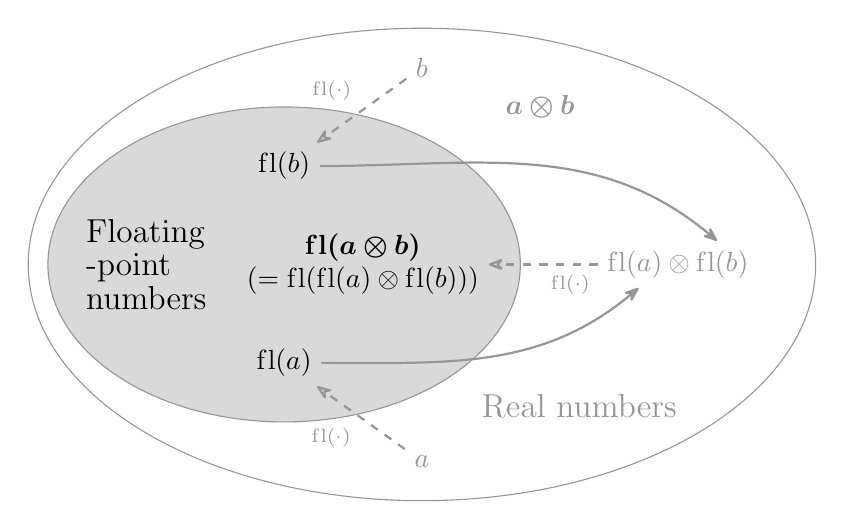
\begin{tikzpicture}[fg]
    \draw (0,0) ellipse (5 and 3);
    \draw[fill=gray!30] (-1.75,0) ellipse (3 and 2);

    \node[align=left] at (2,-1.8) {\large Real numbers};
    \node[align=left] at (-3.5,0) 
        {\large\color{black} Floating\\\large\color{black} -point\\\large\color{black} numbers};

    \node[align=center,black] (fla) at (-1.75,-1.25) {$\fl(a)$};
    \node[align=center] (a) at (0,-2.5) {$a$}; 
    \path[-{Stealth[open,round]},dashed,thick] (a) edge node[below left] 
        {\scriptsize $\fl(\cdot)$} (fla);

    \node[align=center,black] (flb) at (-1.75,1.25) {$\fl(b)$};
    \node[align=center] (b) at (0,2.5) {$b$};
    \path[-{Stealth[open,round]},dashed,thick] (b) edge  node[above left] 
        {\scriptsize $\fl(\cdot)$} (flb);

    \node[align=center] (flab) at (3.25,0) {$\fl(a) \otimes \fl(b)$};
    \path[-{Stealth[round]},thick] (fla) edge [out=0, in=-140] 
        ($(flab)+(-0.5,-0.3)$);
    \path[-{Stealth[round]},thick] (flb) edge [out=0, in=140] 
        ($(flab)+(0.5,0.3)$);

    \node[align=center,black] (flflab) at (-0.75,0) {$\bm{\fl(a \otimes b)}$ \\ 
    $(=\fl(\fl(a) \otimes \fl(b)))$};
    \path[-{Stealth[open,round]},dashed,thick] (flab) edge 
        node[below,near start] {\scriptsize $\fl(\cdot)$} (flflab);

    \node[align=center] (ab) at (1.5,2) {$\bm{a\otimes b}$};
\end{tikzpicture}
\end{document}
